\section{Computational Methods and Software}
\label{sec:software}

% \begin{itemize}
%  \item \st{discretized equations, finite elements, stabilized}
%  \item penalty formulation, also consider discussing sep model
%  \item \st{software (GRINS+Libmesh)}
%  \item \st{verification of software}
%  \item \st{tool-chain, simulation machine and hardware}
%  \item \st{simulation geometry and boundary conditions for wind/thermal-only}
% \end{itemize}

\subsection{Discretization Scheme}

To instantiate the Navier-Stokes equations on computer, we utilize a
Galerkin finite element discretization (FEM), with linear basis functions for
both the velocity and pressure. Unlike the typical FEM formulations,
this scheme circumvents the Babuska-Brezzi conditions and permits use of
equal-order elements for velocity and 
pressure. This is accomplished through the introduction of a
stabilization term first described by Hughes\cite{Hughes198685} and
expanded to a natural convection domain (with sane choices of
stabilization parameters) by Becker and Braack\cite{Becker2002428}. 

Newton iterations are then used for solving the nonlinear problem. 
The resulting system of ODEs are discretized in time using a theta-method. 
The unsteady solver used is typically backward Euler for the corresponding
stability regardless of timestep size. 

\subsection{Penalty Method Implementation}
\todo{write me!}
Talk about penalty method here
cite babuska
cite immersed bounday methods?


\subsection{Simulation Geometry and Boundary Conditions}

%
% be sure to mention the 'sponge' layer. would also be nice to have
% references to papers on it! 
%


All simulations are perfomed in a cuboid domain, with 6 faces. We
utilize a uniform mesh in the lateral directions, and a non-uniform mesh
in height to resolve the boundary layer. The meshes are scaled by system
diameter. So the same number of grid points are used for every
simulation, with the total domain extents scaled up with system size. In
this way the ratio of the domain diameter to system diameter remains
fixed. Likewise, the diffusivities are proportionally scaled with grid
size in order to ensure that the cell Reynolds number is maintained for
every simulation. After operation, solutions are evaluated to ensure
that the qualitative character of the solution does not change. 


%
%explain how cell reynolds number is maintained for each grid
%

For the ``thermal-only'' case study (no mean wind), the simulation
utilizes periodic boundary conditions on the four sides, a modified
neumann condition on the top boundary, and dirichlet boundary conditions
on the bottom (the ground). These are shown schematically in Figure
\ref{fig:thermalbc}. On the ground, a ``no-slip'' velocity boundary
condition is imposed on the velocity field, and a dirichlet condition
uniformly fixes the temperature of the surface. 

The modified neumann condition is necessary due to the precence of both
inflow and outflow across the face. In the region approximately above
the vanes, the concentrated hot plume is lifted by buoyancy
upward and out of the simulation domain. However, the radial inflow
towards the apparatus is drawn in by large scale convection cells larger
than the system diameter. Thus, our boundary conditions must permit
inflow along the areas above and external to the vanes. To prevent the
problem being ill-posed, the ``v'' and ``u'' components of inflow
velocity are set to zero. 

Finally, a ``sponge layer'' is labeled near the top boundary. This layer
artificially increases the momentum diffusivity by ten times the nominal
value. This was designed in response to instabilities in the modified
neumann boundary condition that occured when small, high velocity fluid
parsels would exit the top. This would create high velocity inflows, and
the feedback loop would result in numerical blow-up. Mindful of the fact
that the character of solution not important in this region, and that
our physical interest remains focused on the region inside and
in immediate proximity to the vanes, we introduced a higher diffusivity
``sponge'' region that would diffuse the high velocity exiting jets
sufficiently to prevent numerically un-physical behavior. 

\begin{figure}[!htb]
  \begin{center}
    \includegraphics[width = 8 cm]{figs/thermal_only}
    \caption{Boundary conditions for the thermal-only scenario. }
    \label{fig:thermalbc}
  \end{center}
\end{figure}

The wind cases are diagrammed in figures \ref{fig:windstream} and
\ref{fig:windspan}. The wind case has a proscribed inlet boundary layer
for both the temperature profile as well as the velocity. The velocity
boundary layer is set to the common 7th power function for a
turbulent boundary layer,  
\begin{equation*}
  u_{in}(z) = U \text{ min }\left(\left(\frac{z}{\delta}\right)^7,1\right)
\end{equation*}
where $\delta$, the boundary layer thickness, is set based on data
measured by our experimental partners in the field. 
The thermal boundary layer is assumed to have a similar boundary layer,
but, as observed in real atmospheric flows, there remains a vertical
temperature gradient outside the thin boundary layer. Based on
literature a $2/3$ Kelvin per meter gradient has been
selected\cite{}. The sides, outflow and top are all set to modified
neumann boundary conditions, as described above. The outflow region in
the back also needs the modified neumann as it does occassionally
exhibit mild inflow on account of the unsteady wake. Sponge layers are
set along the top and back of the box. 

%
%335+18*tanh(-z/0.1)-z*2/3
%
\begin{figure}[!htb]
  \begin{center}
    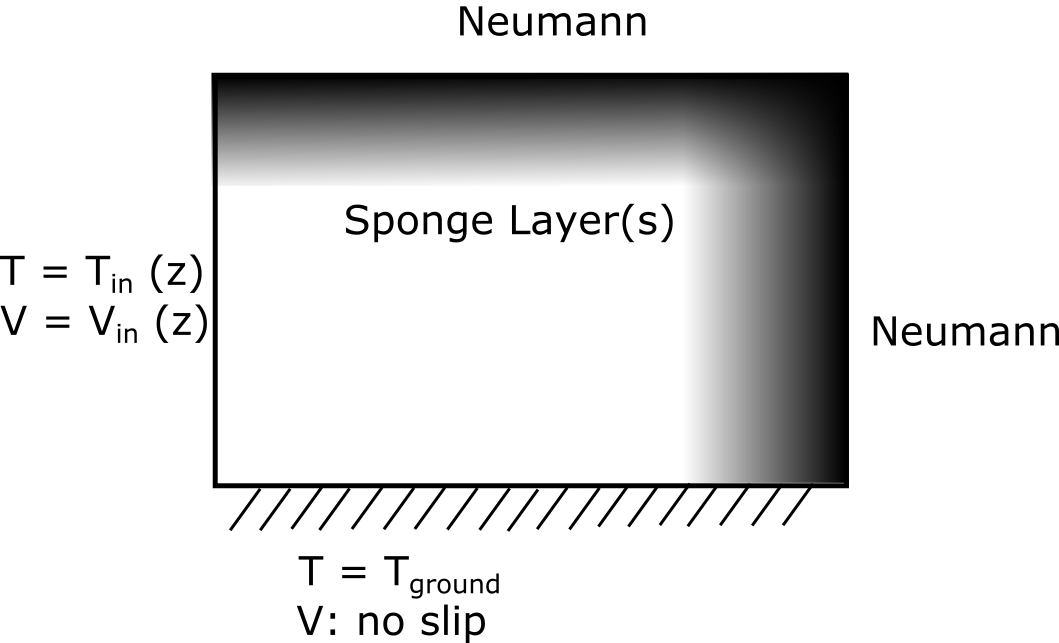
\includegraphics[width = 8 cm]{figs/wind_streamwise}
    \caption{Boundary conditions for the wind and thermal scenario, in
   the streamwise direction.} 
    \label{fig:windstream}
  \end{center}
\end{figure}

\begin{figure}[!htb]
  \begin{center}
    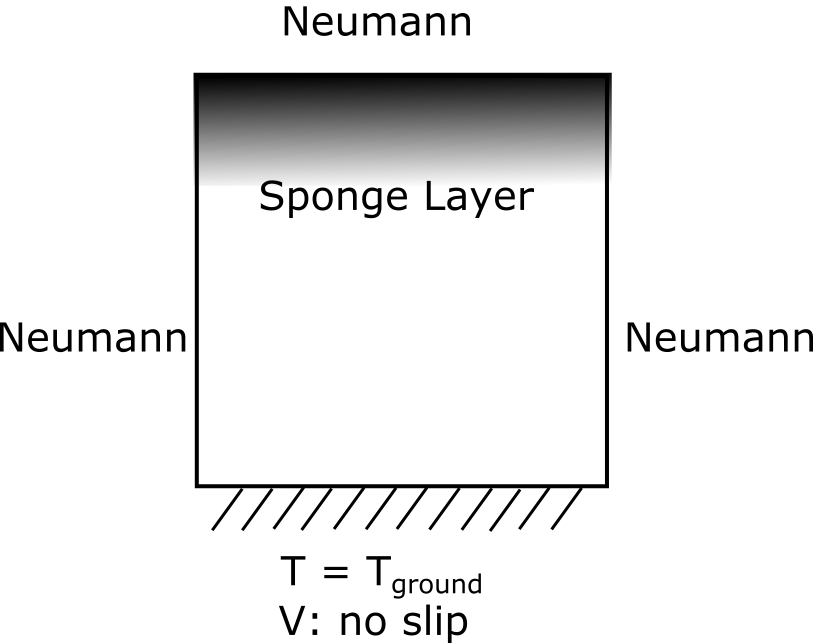
\includegraphics[width = 8 cm]{figs/wind_spanwise}
    \caption{Boundary conditions for the wind and thermal scenario, in
   the spanwise direction. } 
    \label{fig:windspan}
  \end{center}
\end{figure}


\subsection{Software}

A natural choice for FEM software is the
libMesh\cite{libMeshPaper}. Libmesh provides a wide set of tools with
which to build a mesh-based application. However, originally libMesh
applications were required to reimplement many kernels common to finite
element applications, including assembly loops, time integration
schemes, etc.  

We therefore utilize the GRINS library\cite{GRINSpaper}.
GRINS was designed to support multiphysics FEM
applications, the reusability and extensibility of mathematical
modeling kernels, supporting interfaces to existing solver and
discretization libraries to enable modern solution strategies, while, at
the same time, retaining flexibility to effectively tackle the science
or engineering problem of focus. 

GRINS provides a platform that enables powerful numerical algorithms
such as adjoint-based AMR, adaptive modeling, sensitivity analysis,
and, eventually, enabling uncertainty quantification.

GRINS stands for, ``General Reacting Incompressible Navier-Stokes'',
which roughly encapsulates the physical regimes it was originally
designed to simulate. GRINS is open-source, and available on
\hyperref[www.github.com/grinsfem/grins]{github}. It is released 
under LGPL2.1.  

%The remainder of this subsection is devoted to
%discussing the underlying libraries used and the description of the
%GRINS framework.  
% PETSC\cite{petsc} trilinos\cite{trilinos}

% GRINS also utilizes the fparser\cite{fparser}
% library to support both parsing and compilation of mathematical
% functions into high 
% performance kernels. This capability allows for easy specification of
% boundary conditions, initial conditions, or constitutive equations from an input file. 

% Currently, libMesh has been scaled tens of thousands of cores and has
% been run on over 100,000 cores on the BG/Q machine Mira at Argonne National
% Lab\cite{libmesh-scaling}

%In principle, alternative software libraries/frameworks such as
%FEniCS\cite{fenics}, OpenFOAM\cite{openfoam}, etc. would likely be
%capable of simulating this regime. 


\subsection{Tool Chain and Simulation Custodianship}

Runs are queued on Texas Advanced Computing Center (TACC)
supercomputer's Lonestar Four and Stampede. Run durations are typically  
twelve hours to perform several hundred timesteps. 
These runs are generally submitted to the production queue and are  
264-528 processing cores, 
or 22-44 nodes on lonestar (with 12 cores per node), and a similar number
for Stampede. The runs typically have several million degrees of freedom (DoF), 
and thus the local (per core) DoF maintained at $O(10^4)$. This was selected due to 
memory considerations and after a strong scaling analysis of the codebase on these 
resources, as well as consulting with the software primary developers. 

After a run terminates, several worker scripts are automatically invoked. 
These scripts automatically archive the run (outside of the volatile /scratch 
production directories) and simultaneously, label the concluded run with
unique metadata that defines the system environment, the jobs input
files and run definitions, as well as information detailing the
hypothesis or physics the job was intended to investigate. Finally, once
a week an rsync is performed on the entire archived database to ensure
more than single redundancy for the runs. 

In other words, the workflow is sufficiently advanced as to permit
rapidly queuing a series of runs (in parallel) that are intended to
investigate a variety of conditions or scenario parameters. This
capabilty is necessary for the optimization campaign detailed in
\ref{sec:proposed_work}, where running many concurent investigations
will be required to adaquetly sample the configuration space. 
